\documentclass[a4paper]{article}
\usepackage[T1,T2A]{fontenc}
\usepackage[russian]{babel}
\usepackage{amsmath, amsfonts, amssymb}
\usepackage[lmargin=5mm, rmargin=5mm, tmargin = 2cm, bmargin = 1.5cm]{geometry}
\usepackage{emptypage}
\input{~/.preamble.tex}

\begin{document}
\begin{titlepage}
  \Large
  \begin{center}
    Санкт-Петербургский\\
    Политехнический университет Петра Великого\\
    \vspace{10em}
    Отчёт по курсовой работе\\
    \vspace{2em}
    \textbf{Сравнение решения задач интерполирования изученными методами}
  \end{center}
  \vspace{6em}
  \begin{flushright}
    Студент: Копнов Александр Александрович\\
    Преподаватель: Добрецова Светлана Борисовна\\
    Группа: 5030102/00003
  \end{flushright}
  \vspace{\fill}
  \begin{center}
    Санкт-Петербург\\
    2022
  \end{center}
\end{titlepage}

\section{Задание}\label{sec:task}
Приблизить табличную функцию на равномерной сетке
\begin{enumerate}
\item\label{item:1} интерполяционным полиномом в форме Ньютона слева-направо
\item кубическим интерполяционным сплайном
\end{enumerate}
Сравнить результаты по графикам ошибок на отрезке для малого числа узлов. Исследовать зависимость нормы ошибки от класса
гладкости исходной функции.
\section{Постановка задачи}\label{sec:formal}

Дана сетка \(x^{h} := \{x_{i}\}^{n}_{i=0}\) и сеточная функция \(y^{h} := \{y_{i}\}_{i=0}^{n}\). Необходимо приблизить
фукнцию \(y(x)\) функцией \(\phi(x)\) так, что \[
  \phi(x_{i}) = y_{i}, \quad i = \overline{1,n}
\]
\section{Предварительный анализ}\label{sec:analysys}
\begin{enumerate}
        \item Приближая интерполяционным полиномом, задача построить полином \(\phi(x)\), удовлетворяющий критерию близости \[
        \phi(x_{i}) = y_{i}, \quad i = \overline{0,n}
        \]
  \item Приближая сплайном, необходимо найти сплайн \[
        S = \{ P_{i}(x) : P_{i}(x_{i}) = y_{i}, P_{i}(x_{i-1}) = y_{i-1} \quad i = \overline{1,n}; x \in [x_{i-1}; x_{i}]\}
        \]\[
        P_{i} = a_{i}x^{3}+b_{i}x^2+c_{i}x + d_{i}
        \]\[
        S \in C^{2} \quad (P'_{i}(x_{i}) = P'_{i+1}(x_{i}), P''_{i}(x_{i}) = P''_{i+1}(x_{i}) \quad i = \overline{1,n})
        \]\[
        P'_{1}(x_0) = f'(a) \quad P'_{n}(x_{n}) = f'(b)
        \]
\end{enumerate}
\section{Алгоритмы}\label{sec:algo}
\subsection{Интерполяционный полином в форме Ньютона слева-направо}\label{subsec:Newton}
\textbf{Условия применимости}:
\begin{enumerate}
\item\label{item:3} Все узлы сетки \(x^{h}\) попарно различны
  \item степень искомого полинома на единицу меньше, чем кол-во точек
\end{enumerate}
Для построения полинома требуются разделённые разности. \(y(x_0,\ldots,x_{i})\) --- разделённая разность \(i\)-го порядка. \[
  y(x_{k_{0}},\ldots,x_{k_{m}}) = \frac{y(x_{k_{1}},\ldots,x_{k_{m}}) - y(x_{k_{0}},\ldots,x_{k_{m-1}})}{x_{k_{m}}-x_{k_{0}}}
\]В частности \[
  y(x_{0},\ldots,x_{i}) = \frac{y(x_{1},\ldots,x_{i})-y(x_{0},\ldots,x_{i-1})}{x_{i}-x_{0}}
\]
Если представить разделённые разности в виде таблицы \[
  \begin{matrix}
    & 1 \text{пор.} & 2 \text{пор.} & & n-1 \text{пор.} & n \text{пор.} \\
    y_0 & y(x_0,x_1) & y(x_0,x_1,x_2) & \vdots & y(x_0,x_1,\ldots,x_{n-1}) & y(x_0,x_1,\ldots,x_{n})\\
    y_1 & y(x_1,x_2) & y(x_1,x_2,x_3) & \vdots & y(x_1,x_2,\ldots,x_{n}) \\
    \ldots & \ldots \\
    y_{n-1} & y(x_{n-1},x_{n})\\
    y_{n}
  \end{matrix}
\]
Для полинома Ньютона слева-направо нужны все разности из первой строки.\\
Вычислять разности удобно по столбцам: \[
  y(i,j) = \frac{y(i,j-1)-y(i+1,j-1)}{x(i)-x(i+j)} \quad j = \overline{1,n}, i = \overline{0,(n-j)}
\]
Сам интерполяционный полином имеет вид \[
  P_{n}(x) = y_0 + (x-x_0)y(x_0,x_1)+\cdots+(x-x_0)(x-x_1)\cdots(x-x_{n-1})y(x_0,\ldots,x_{n}) = \sum_{i=0}^n y(x_0,x_1,\ldots,x_{i}) \prod_{k=0}^{i-1} (x-x_{k})
\]
\textbf{Теоретическая оценка результатов}\\
Пусть \(\{x_{i}\}_{i=0}^{n}\) --- узлы интерполяции, \(x \neq x_{i}\) --- точка, в которой производится оценка. Добавим \(x\) к
узлам интерполяции. \[
  P_{n+1}(x) = y
\]\[
  P_{n+1}(x) = P_{n}(x) + y(x_0,\ldots,x_{n},x)\omega(x)
\]\[
  R_{n}(x) = y-P_{n}(x) = y(x_0,\ldots,x_{n},x)\omega(x)
\]
Ошибка зависит от значений производной исходной функции на отрезке, количества узлов и их расположения. \[
  \abs{y - P(x)} = \abs{f^{(n+1)}(\eta)} \frac{\omega_{n+1}(x)}{(n+1)!}
\]
Если функция принадлежит классу гладкости \(C^{k}\), нет информации о \(k+1\) и следующих производных. Соответственно
нет оценки для полинома степени \(k\) и более.
\subsection{Кубический интерполяционный сплайн}\label{subsec:spline}
\textbf{Условия применимости}:
\begin{enumerate}
\item\label{item:2} Все узлы сетки \(x^{h}\) попарно различны
  \item Сетка \(x^{h}\) является упорядоченной
\end{enumerate}
Для корректной оценки точности сплайна функция должна принадлежать классу \(C^{4}\).

Необходимо найти \(4n\) коэфициентов для \(n\) функций \[
  P_{i} = a_{i}x^{3}+b_{i}x^2+c_{i}x + d_{i} \quad x \in [x_{i-1}]
\]
Требуется \(4n\) условий. Из формулировки задачи условия непрерывности до второй производной для внутренних точек \[
  \begin{cases}
    P_{i}(x_{i}) = P_{i+1}(x_{i})\\
    P_{i}'(x_{i}) = P_{i+1}'(x_{i})\\
    P_{i}''(x_{i}) = P_{i+1}''(x_{i})\\
  \end{cases} \quad  i = \overline{1,n-1}
\]
Также имеем условия интерполирования \(P_{1}(x_{0}) = y_{0}\) и \(P_{i}(x_{i})=y_{i}\) для \(i = \overline{1,n}\).
Добавив граничные условия \(P_{1}'(x_{0}) = y'(x_{0})\) и \(P_{n}'(x_{n}) = y'(x_{n})\) мы можем решить систему
уравнений.

Так как \(P\) --- полином третьей степени, \(P''\) --- линейная функция. Задав
\(P''_{i}(x_{i}) = M_{i},P''_{i}(x_{i-1}) = M_{i-1}\), имеем \[
  P_{i}''(x) = M_{i-1} \frac{x_{i}-x}{h_{1}} + M_{i} \frac{x-x_{i-1}}{h_{i}} \quad x \in [x_{i-1},x_{i}] \quad h_{i} = x_{i} - x_{i-1}
\]
Дважды проинтегрировав, получаем \[
  P' = M_{i} \frac{(x-x_{i-1})^2}{2h_{i}} - M_{i-1} \frac{(x_{i}-x)^2}{2h_{i}} + C
\]\[
  P = M_{i-1} \frac{(x_{i}-x)^{3}}{6h_{i}} + M_{i} \frac{(x-x_{i-1})^{3}}{6h_{i}} + C_{i}(x-x_{i-1}) + \tilde{C}_{i}
\]
Из граничных условий имеем \[
  P_{1}'(x_{0}) = -M_{0} \frac{h_1}{2} + \frac{y_1-y_0}{h_1} - \frac{h_1}{6}\left(M_1-M_0\right) = f'(a)
\]\[
  P_{n}'(x_{n}) = M_{n} \frac{h_{n}}{2} + \frac{y_{n}-y_{n-1}}{h_{n}} - \frac{h_{n}}{6} \left( M_{n} - M_{n-1} \right) = f'(b)
\]
Из условия непрерывности первых производных получаем \[
  \frac{h_{i}}{h_{i}+h_{i+1}} M_{i-1} + 2M_{i} + \frac{h_{i}}{h_{i}+h_{i+1}}M_{i+1} =
  \frac{6}{h_{i}+h_{i+1}}\left( \frac{y_{i+1}-y_{i}}{h_{i+1}} - \frac{y_{1}-y_{i-1}}{h_{i}}\right) \quad i = 1,\ldots,n-1
\]
Совокупность этих условий даёт трёхдиагональную СЛАУ \[
\begin{pmatrix}
  c_0 & d_0 & 0 & 0 & \ldots & 0 & 0 & 0\\
  b_1 & c_1 & d_1 & 0 & \ldots & 0 & 0 & 0\\
  0 & b_2 & c_2 & d_2 & \ldots & 0 & 0 & 0\\
  \ldots & \ldots & \ldots & \ldots & \ldots & \ldots & \ldots & \ldots\\
  0 & 0 & 0 & 0& \ldots &b_{n-1} & c_{n-1} & d_{n-1}\\
  0 & 0 & 0 & 0 & \ldots & 0 & b_n & c_n \\
\end{pmatrix}
\begin{pmatrix}[c]
  M_0 \\ M_1 \\ M_2 \\ \vdots \\ M_{n-1} \\ M_{n}
\end{pmatrix}
= \begin{pmatrix}[c]
    r_0 \\ r_1 \\ r_2 \\ \vdots \\ r_{n-1} \\ r_{n}
  \end{pmatrix}
\]
Для решения можно использовать метод прогонки:
\begin{enumerate}
  \item Предположим, существуют \(\delta_{i},\lambda_{i}\), такие, что \(M_{i} = \delta_{i}M_{i+1}+\lambda_{i}\).\\
        Уменьшив индекс на единицу (\(M_{i-1} = \delta_{i-1}M_{i} + \lambda_{i-1}\)) подставим в уравнение системы: \[
        b_{i}\delta_{i-1}M_{i} + b_{i}\lambda_{i-1}+c_{i}M_{i}+d_{i}M_{i+1} = r_{i}
        \]
        Получаем \[
        M_{i}=-\frac{d_{i}}{c_{i}+b_{i} \delta_{i-1}} M_{i+1}+\frac{r_{i}-b_{i} \lambda_{i-1}}{c_{i}+b_{i} \delta_{i-1}}
        \]
  \item В силу условия \(b_{0} = 0\) процесс вычисления \(\delta,\lambda\) начинается со значений \[
        \delta_{0} = -\frac{d_0}{c_0} \quad \lambda_{0} = \frac{r_{0}}{c_{0}}
        \]
  \item Продолжаем вычисления по рекуррентным выражениям для \(\delta,\lambda\): \[
        \delta_{i}=-\frac{d_{i}}{c_{i}+b_{i} \delta_{i-1}}, \quad \lambda_{i}=\frac{r_{i}-b_{i} \lambda_{i-1}}{c_{i}+b_{i} \delta_{i-1}} \quad i=\overline{1,n}
        \]
        Причём при \(i=n\) в силу \(d_{n} = 0\) получим \(\delta_{n}=0\). Следовательно \(M_{n} =\lambda_{n}\).
  \item Находим значения \(M_{i}\) при \(i=\overline{n-1,0}\) по формуле \(M_{i-1} = \delta_{i-1}M_{i} + \lambda_{i-1}\)
\end{enumerate}

После решения СЛАУ, константы находятся из условий для границ отрезков по формулам \[
  P_{i}(x_{i-1}) = y_{i-1} = M_{i-1} \frac{h_{i}^2}{6} + \tilde{C}_{i} \quad \tilde{C}_{i} = y_{i-1} - M_{i-1} \frac{h_{i}^2}{6}
\]\[
  P_{i}(x_{i}) = y_{i} = M_{i} \frac{h_{i}^2}{6} + C_{i}h_{i} + \tilde{C}_{i} \quad C_{i} = \frac{y_{i}-y_{i-1}}{h_{i}} - \frac{h}{6} (M_{i} - M_{i-1})
\]
\textbf{Теоретическая оценка результатов}\\
Если \(f \in C^{4}([a,b])\) и \(S\) --- кубический интерполяционный сплайн для функции \(f\), то \[
  \forall x \in [a,b] \abs{f(x)-S(x)} \leq Ch^{4}
\]
где \(h = \max_{i}\ h_{i}\) и \(C = \frac{5}{384} \max_{x\in[a,b]}\abs{f^{(4)}(x)}\)
\section{Контрольные тесты}\label{sec:tests}
Были исследованы  функции \(f(x) = ctg x + x^{2}\) и \(g(x) = f(1.7) + \abs{f(x) - f(1.7)}\) на отрезке \([1,2.5]\).
Генерировались сетки на 4,6 и 8 точек, для которых были построены полные графики ошибки на отрезке и сетки на
\(n = \overline{4,51}\) точках, используемые для графика зависимости максимальной ошибки от количества точек.
\section{Численный анализ}\label{sec:numAn}
\begin{center}
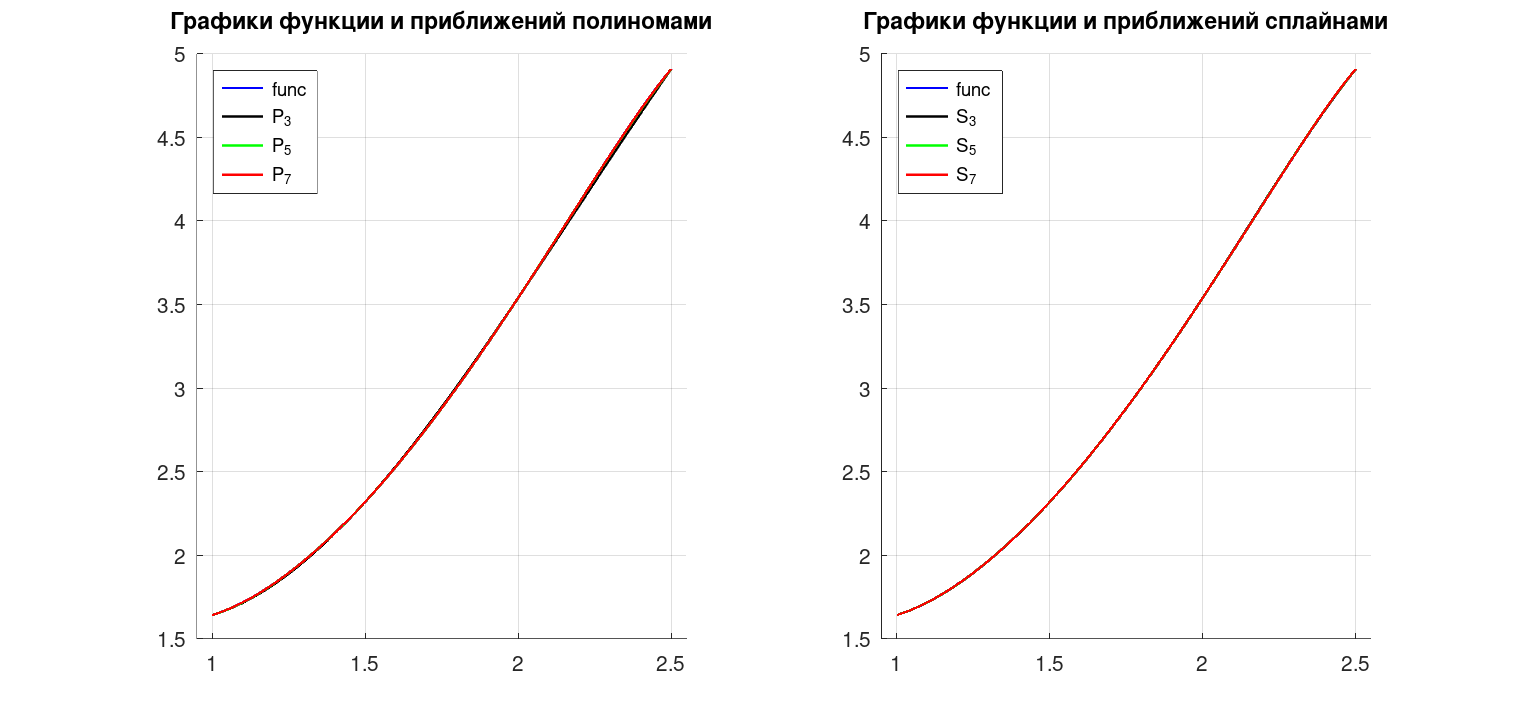
\includegraphics[width=\textwidth]{compGraph.png}
\end{center}
\begin{center}
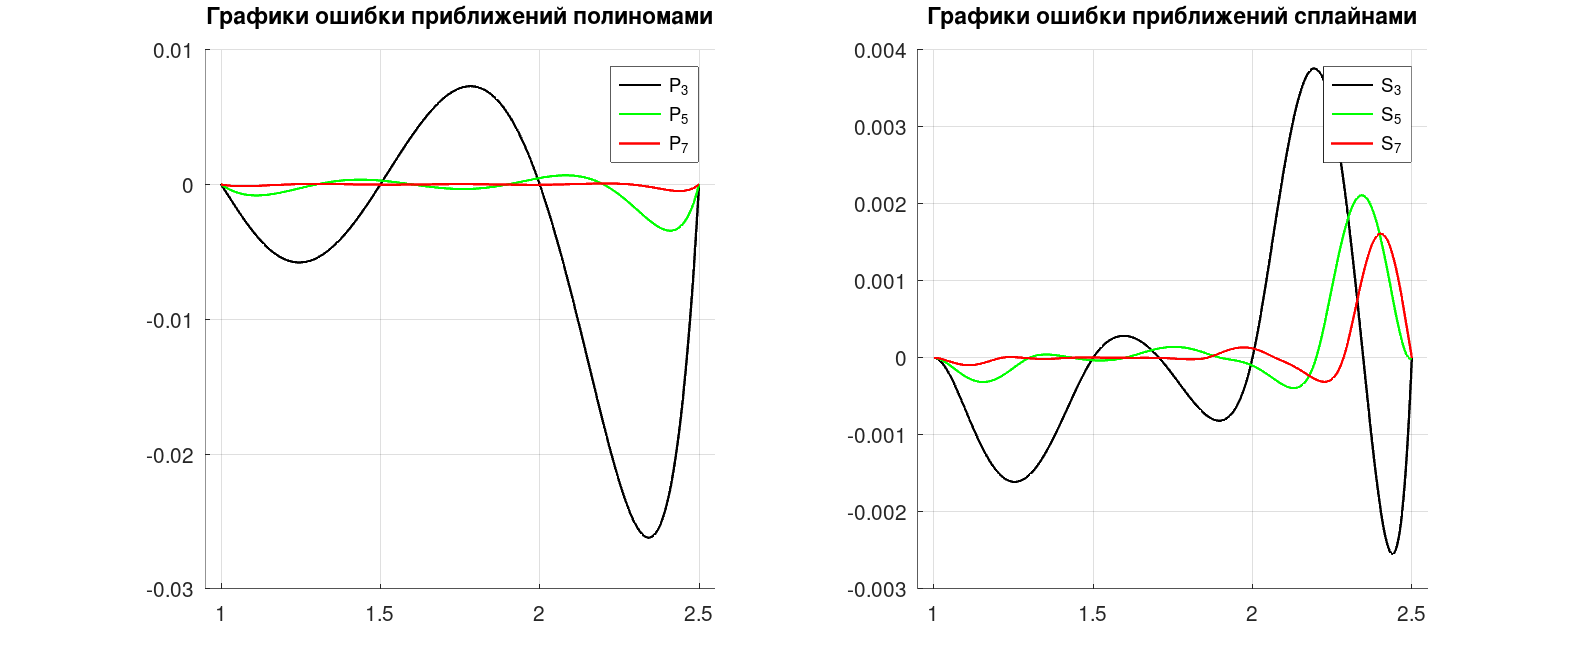
\includegraphics[width=\textwidth]{compErr.png}
\end{center}

В обоих случаях ошибка равна нулю в узловых точках, меняя знак при переходе через них.

При приближении полиномом ошибка максимальна у границ отрезка.

При приближении сплайном ошибка максимальна на правой границе, что может быть связано с выбором направления прогонки. На
некоторых частях отрезка ошибка меняет знак в середине.

\begin{center}
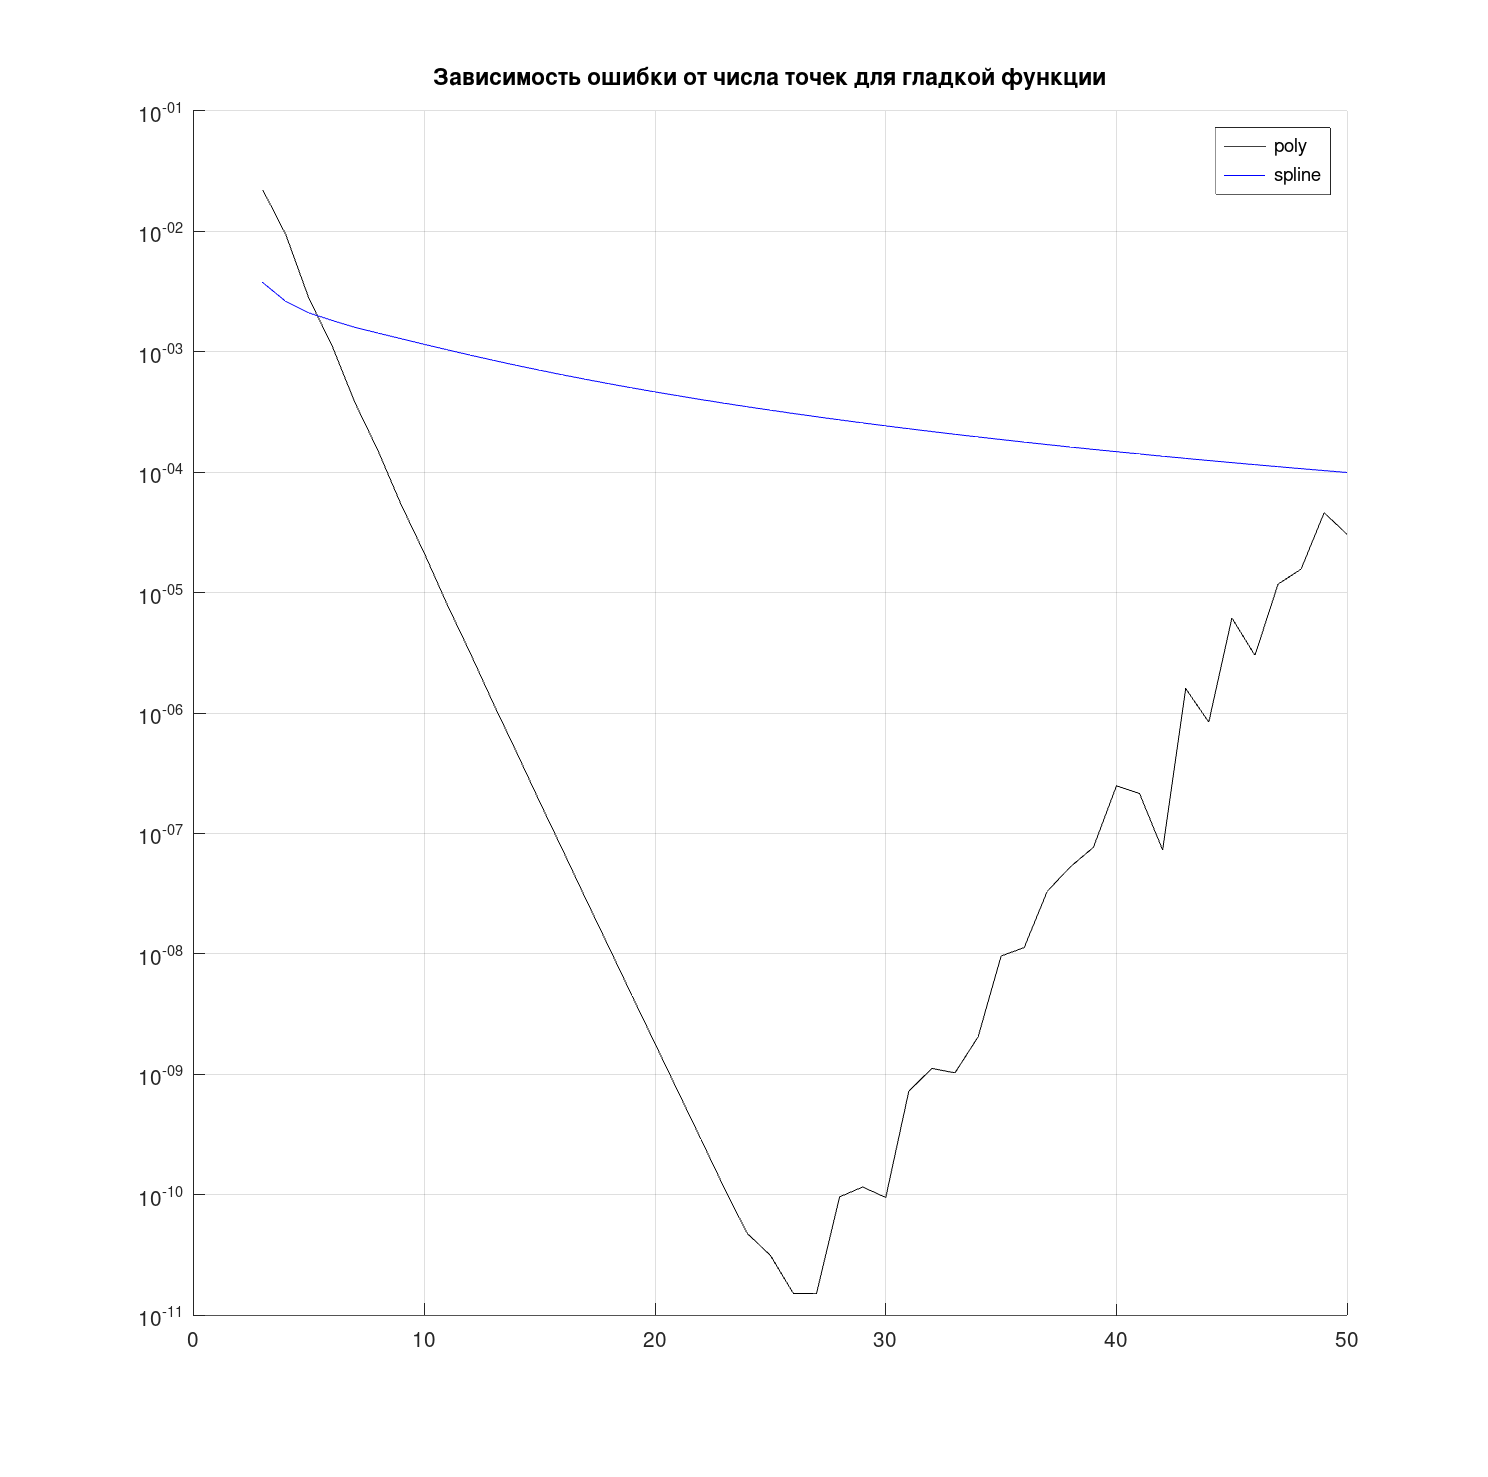
\includegraphics[width=0.7\textwidth]{err(n).png}
\end{center}
При изменении числа точек ошибка сплайна монотонно уменьшается, однако достигаемая точность намного меньше, чем точность
приближения полиномом.

При приближении полиномом ошибка быстро убывает до 25 точек, затем начинает
возрастать со скоростью примерно на четверть меньше.
\begin{center}
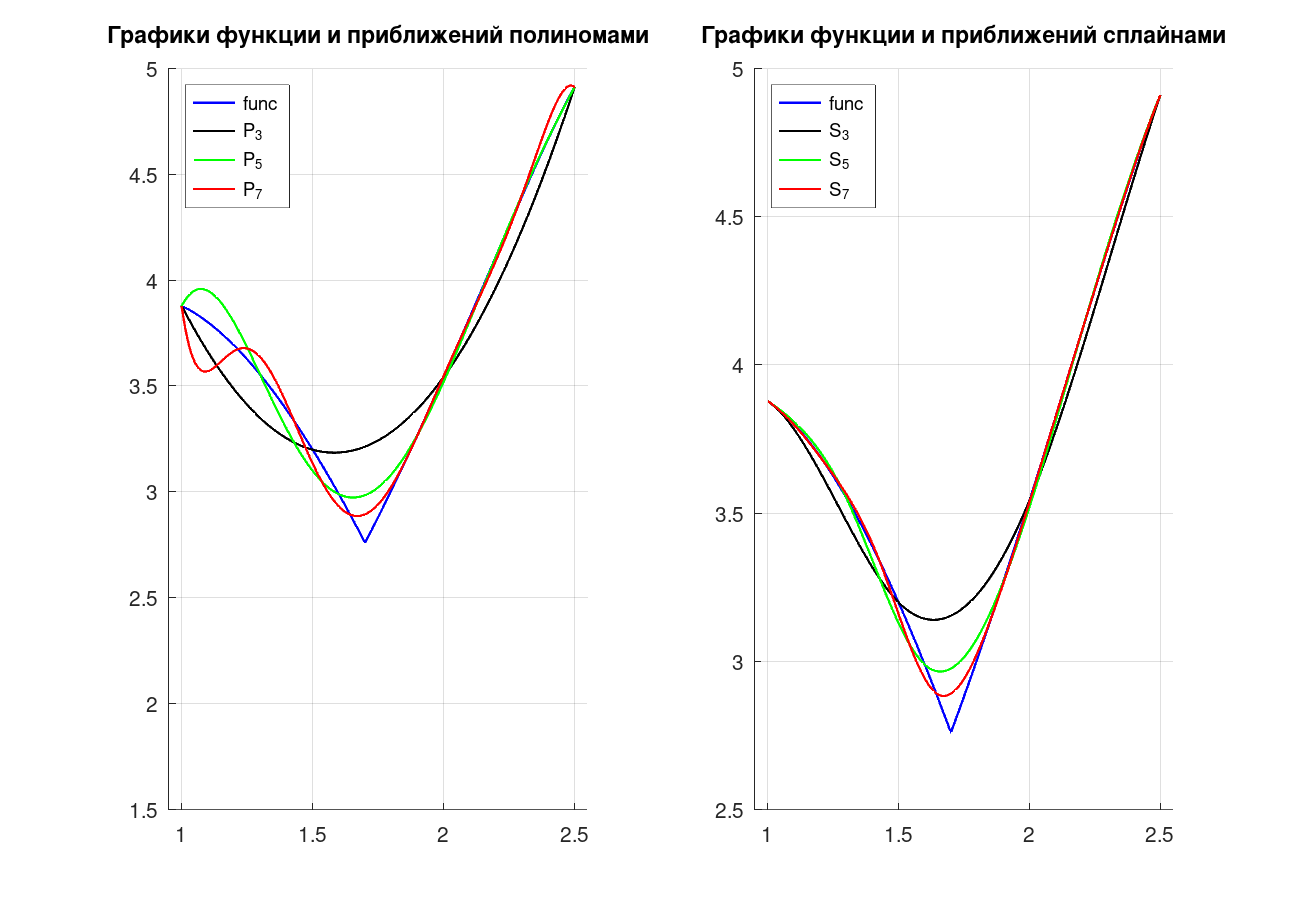
\includegraphics[width=0.9\textwidth]{compGraphG.png}
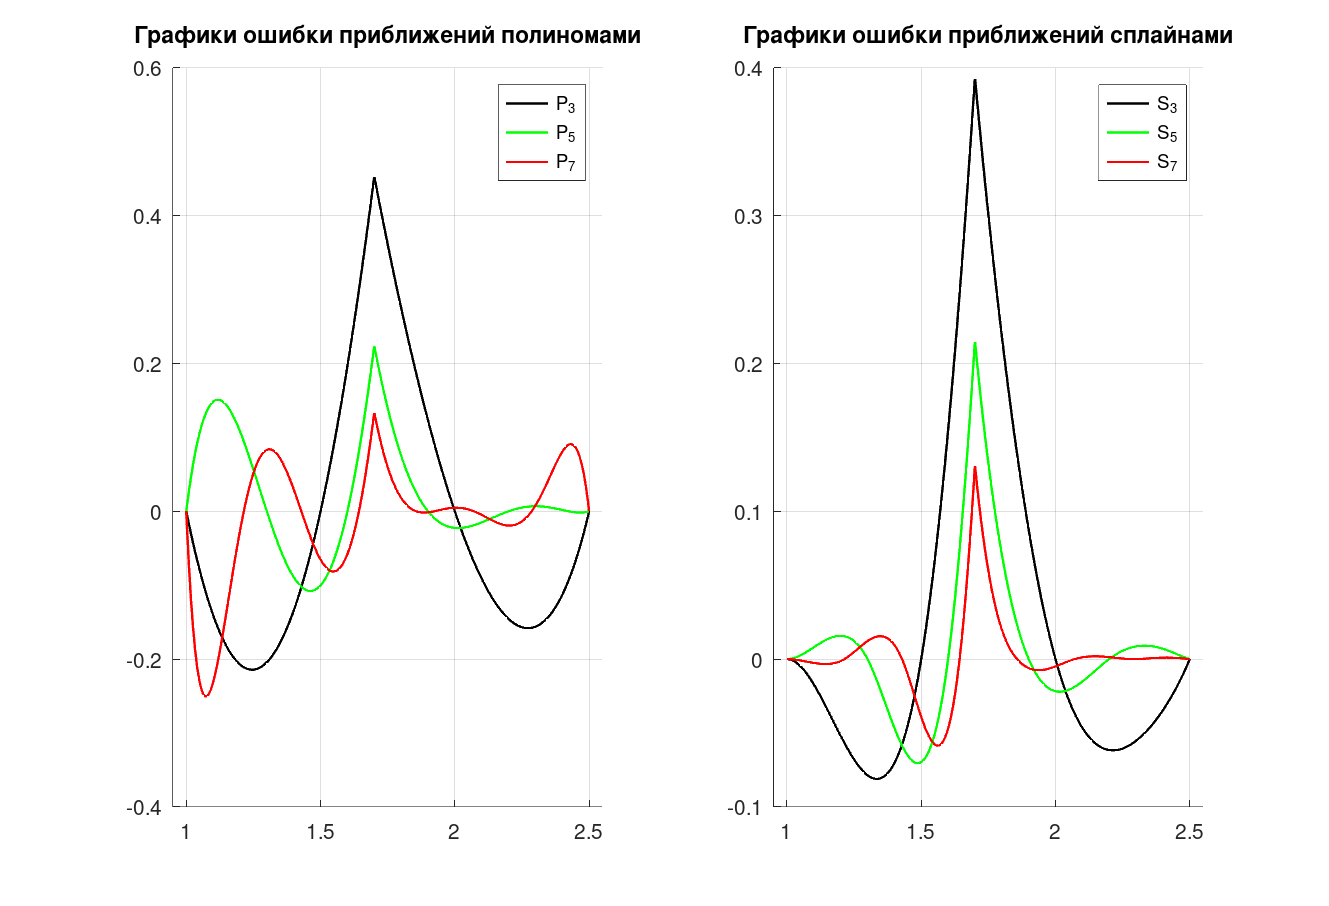
\includegraphics[width=0.9\textwidth]{compErrG.png}
\end{center}
Ошибка интерполяционного полинома максимальна в точке разрыва для третьей степени, но более высокие степени лучше
приближают разрыв за счёт возмущений у границ. При увеличении степени относительная величина ошибки в точке разрыва
становится меньше, и к 7 степени полинома максимум достигается уже на левой границе.

При приближении сплайном максимум ошибки достигается в точке разрыва, но аномальное поведение функции слабо влияет на
поведение ошибки на других отрезках разбиения.
\begin{center}
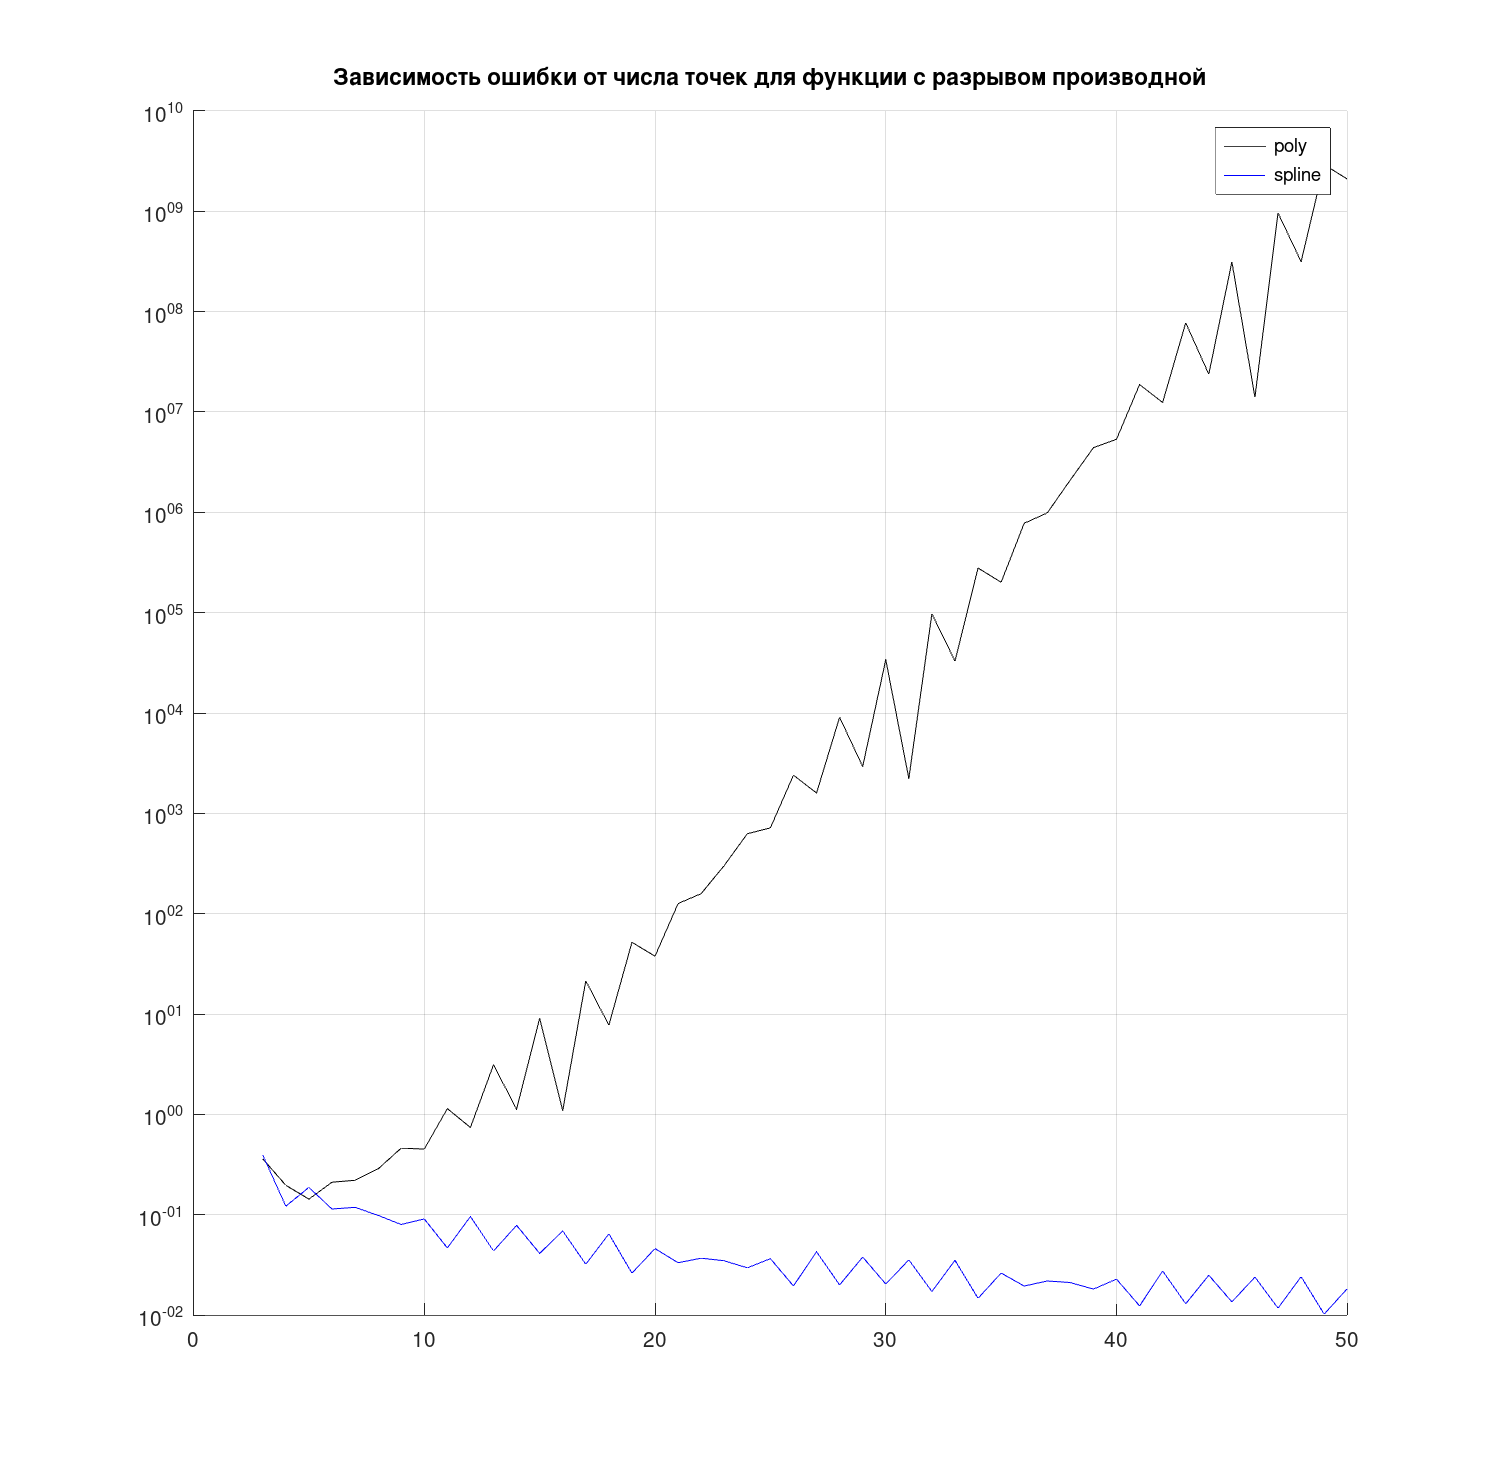
\includegraphics[width=0.7\textwidth]{err(k).png}
\end{center}

Периодические колебания ошибки, заметные на обоих графиках связаны с положением разрыва внутри отрезка разбиения.

Разрыв в производной оказывает большое влияние на точность интерполяции полиномом, ошибка начинает возрастать уже
примерно на 7 точках вместо 25 для гладкой функции.

Приближение сплайном более точно и ошибка уменьшается, также как и для гладкой функции.

\section{Вывод}\label{sec:res}
Приближение полиномом позволяет достичь большей точности при малом количестве точек, но ошибка начинает быстро
возрастать (при добавлении 3 точек ошибка возрастает примерно на порядок) при измельчении сетки на более чем примерно 25
отрезков. Это связано с нестабильностью корневого полинома \(\omega(x)\) высоких степеней.
Ошибка при приближении полиномом максимальна у границ отрезка и невелика в центре.

Также приближение полиномом накладывает требования на гладкость функции. Если функция имеет разрыв производной, при
увеличении степени полинома выше степени разрыва, ошибка начинает быстро возрастать, что согласуется с формулой для
оценки ошибки \[
  \abs{y - P(x)} = \abs{f^{(n+1)}(\eta)} \frac{\omega_{n+1}(x)}{(n+1)!}
\]
Чтобы хорошо приблизить функцию с разрывом, можно представить её как кусочную функцию из двух разных функций, приближаемых
независимо, что похоже на метод, используемый в сплайнах.

При приближении сплайном достигаемая точность намного меньше, чем точность при использовании полинома, однако при
увеличении количества точек она возрастает и не начнёт убывать, так как нет полиномов высоких степеней, являющихся основным
источником ошибки.

В зависимости от того, меняет ли ошибка знак при переходе через середину, ошибка может достигать локального максимума на
отрезке разбиения в середине всего отрезка или одной из его половин.

Сплайны намного лучше подходят для приближения функции с разрывом, так как влияние разрыва ограничено.

\end{document}
